\chapter{Modeling Human Workload in Unmanned Aerial Systems}\label{ch:workload_paper}
\noindent J. J. Moore, R. Ivie, T.J. Gledhill, E. Mercer and M. A. Goodrich. Modeling Human Workload in Unmanned Aerial Systems. In Proceedings of AAAI 2014 Spring Symposium on Formal Verification \& Modeling in Human-Machine Systems.

\begin{abstract}
%\begin{quote}
Unmanned aerial systems (UASs) often require multiple human operators fulfilling diverse roles for safe correct operation.  Although some dispute the utility of minimizing the number of humans needed to administer a UAS~\cite{MurphyBurke2010}, minimization remains a long-standing objective for many designers.  This paper presents work toward understanding how workload is distributed between multiple human operators and multiple autonomous system elements in a UAS across time, with an ultimate goal to reduce the number of humans in the system. The approach formally models the {\em actors} in a UAS as a set of communicating finite state machines, modified to include a simple form of external memory. The interactions among actors are then modeled as a directed graph.  The individual machines, one for each actor in the UAS, and the directed graph are augmented with workload metrics derived from a review of the relevant literature. The model is implemented as a Java program, which is analyzed by the Java Pathfinder (JPF) model checker, which generates workload profiles over time.  To demonstrate the utility of the approach, this paper presents a case study on a wilderness search and rescue (WiSAR) UAS analyzing two different mission outcomes. The generated workload profiles are shown to be consistent with known features of actual workload events in the WiSAR system. 
%\end{quote}
\end{abstract}

\noindent
\section{Introduction}

Unmanned aerial systems (UASs), ranging from large military-style Predators to small civilian-use hovercraft, usually require more than one human to operate.  It is perhaps ironic that a so-called ``unmanned'' system requires multiple human operators, but when a UAS is part of a mission that requires more than moving from point A to point B, there are many different tasks that rely on human input including: operating the UAS, managing a payload (i.e., camera), managing mission objectives etc.  Some argue that this is desirable because different aspects of a mission are handled by humans trained for those aspects~\cite{MurphyBurke2010}. As human resources are expensive, others argue that it is desirable to reduce the number of humans involved.

This paper explores the open question of {\em how} to reduce the number of humans while maintaining a high level of robustness.  Some progress has been made by improving autonomy using, for example, automatic path-planning~\cite{WongBourgaultFurukawa2005,878915,pettersson2006probabilistic,QuigleyBarberEtAl2005,NelsonBarberMcLainBeard2006}, and automated target recognition~\cite{MorseEnghGoodrich2010,dasgupta2008multiagent,barber2006vision}. However, careful human factors suggest that the impact of changes in autonomy are often subtle and difficult to predict, and this decreases confidence that the combined human-machine system will be robust across a wide range of mission parameters~\cite{KaberEndsley2004,chen2011supervisory,chen2007human}.

The research in this paper argues that one reason for the limitations of prior work in measuring workload is that the level of resolution is too detailed.  For example, although the NASA TLX dimensions include various contributing factors to workload (e.g., physical effort and mental effort), the temporal distribution of workload tends to be ``chunked" across a period of time.  Secondary task measures can provide a more detailed albeit indirect breakdown of available cognitive resources as a function of time~\cite{kaber1999adaptive}, but with insufficient explanatory power for what in the task causes workload peaks and abatement.  Cognitive workload measures, including those that derive from Wickens' multiple resource theory~\cite{wickens2002multiple}, provide useful information about the causes of workload spikes, but these measures have not been widely adopted; one way to interpret the research in this paper is as a step toward robust implementations of elements of these measures.  Finally, measures derived from cognitive models such as ACT-R are providing more low-level descriptions of workload which potentially include a temporal history~\cite{lebiere2013cognitive}, but these approaches may require a modeling effort that is too time-consuming to be practical for some systems.

This paper presents a model of four human roles for a UAS-enabled wilderness search and rescue (WiSAR) task, and is based on prior work on designing systems through field work and cognitive task analyses~\cite{Adams2008,GoodrichMorse2008}.  The paper first identifies a suite of possible workload measures based on a review of the literature.  It then considers seven {\em actors} in the team: the UAV, the operator and the operator's GUI, the video analyst and the analyst's GUI, the mission manager, and a role called the ``parent search'' which serves to connect the UAS technical search team to the other components of the search enterprise.  The paper then presents the formal model of each of these actors using finite state machines, and then discuss how the connections between these state machines defines what is called a {\em Directed Team Graph} (DiTG) that describes who communicates with whom and under what conditions.  The paper then describes how to augment the model to be able to encode specific metrics based on a subset of the measures identified in the literature.  Using the Java PathFinder model checker, a temporal profile is created for each of the workload metrics. These profiles are checked for consistency by associating workload peaks and abatement with likely causes.
 
\section{Workload Categories}

Workload is restricted to three general categories of metrics in this work: cognitive, temporal, and algorithmic.\footnote{A fourth relevant workload category is the cost of maintaining team constructs like shared situation awareness is future work \cite{EliasFiore2011}.}

Cognitive workload describes the difficulties associated with managing various signals, decisions, and actions relevant to a particular task or goal~\cite{MorayEtAl91,lebiere2013cognitive,Goodrich2004,Chadwick2004}. We adopt a simple form of Wickens' multiple resource theory~\cite{wickens2002multiple}, and make the simplifying assumption that cognitive workload can be divided into two categories: parallel sensing and sequential decision making. We further restrict the sensing channels to visual and auditory modalities, ignoring haptic.  Parallel sensing means that it is possible for a human to perceive complementary stimuli over different channels. An example of this would be an individual hearing their call sign on the radio while analyzing video. However, when multiple signals may occur over the same channel at the same time, this induces attentional workload for the human. Sequential decision making occurs when a decision must be made, where we have adopted the assumption made by Wickens and supported by work in the psychology of attention~\cite{Pashler98} that a ``bottle-neck" occurs when multiple channels either (a)~require a decision to be generated or (b)~exceed the limits of working memory. 

Algorithmic workload results from the difficulty of bringing a task to completion. Adopting a common model from artificial intelligence~\cite{Murphy00}, and consistent with Wickens' three stage multiple resource model, we assume that this is comprised of three phases: sense, plan, and act. During the sensing phase, the actor takes all active inputs, interprets them, and generates a set of relevant decision-making parameters. In the planning phase the actor reviews the breadth of choices available and selects one. The actor might use search or a more naturalistic decision-making process like recognition-primed decision-making~\cite{ZsambokKlein97} or a cognitive heuristic~\cite{GigerenzerTodd99}. In the acting phase the actor carries out the decision. Before concluding, we note that workload is highly dependent on the experience of the actor~\cite{ZsambokKlein97}, but we leave a careful treatment of this to future work.

\begin{comment}
We assume that the workload in these two phases is related to the number of choices the actor has, allowing us to use big-O analysis from computational complexity theory to describe the workload associated with sensing and planning; in this paper we make the unrealistic assumption that workload from computational complexity is $O(n)$, but include an explicit temporal component that allows us to detect when multiple decisions ``pile up" at the same time. During the acting phase, the actor either follows through with the decision or disregards it. The workload in this section is entirely dependent on the length and difficulty of executing the plan. 
\end{comment}

Temporal workload deals with the scheduling of prioritized, infrequent, and/or repetitious tasks~\cite{DessoukyEtAl95,MorayEtAl91}. Various measures have been proposed, but we are most interested in those related to so-called ``fan-out", meaning the number of tasks that a single actor can manage \cite{Goodrich2010,OlsenWood2004,CrandallEtAl2005,Cummings2007}. There are two particularly important aspects of temporal workload. First, when a task is constrained by (a)~the time by which the task must be completed or (b)~the need to complete other tasks before or after the given task then (c)~it causes scheduling pressure and workload~\cite{MauDolan2006}. The second aspect is operational tempo, which represents how frequently new tasks arrive.  From a scheduling or queuing theory perspective, operational tempo impacts workload by causing pressure to manage the rate of arrival and the response time of the decision.

\section{Actor Model} 

In previous work~\cite{gledhill2013modelinguas}, we represented each {\em actor}, human or autonomous component, of the WiSAR search team as a Mealy state machines as has been done in other models~\cite{bolton2013litreview}. This work uses Moore machines where output is determined only by present state.

\begin{comment}
\begin{figure}[h]
\center
\setlength{\abovecaptionskip}{1mm}
\setlength{\belowcaptionskip}{1mm}
\setlength{\textfloatsep}{1mm}
\setlength{\floatsep}{1mm}
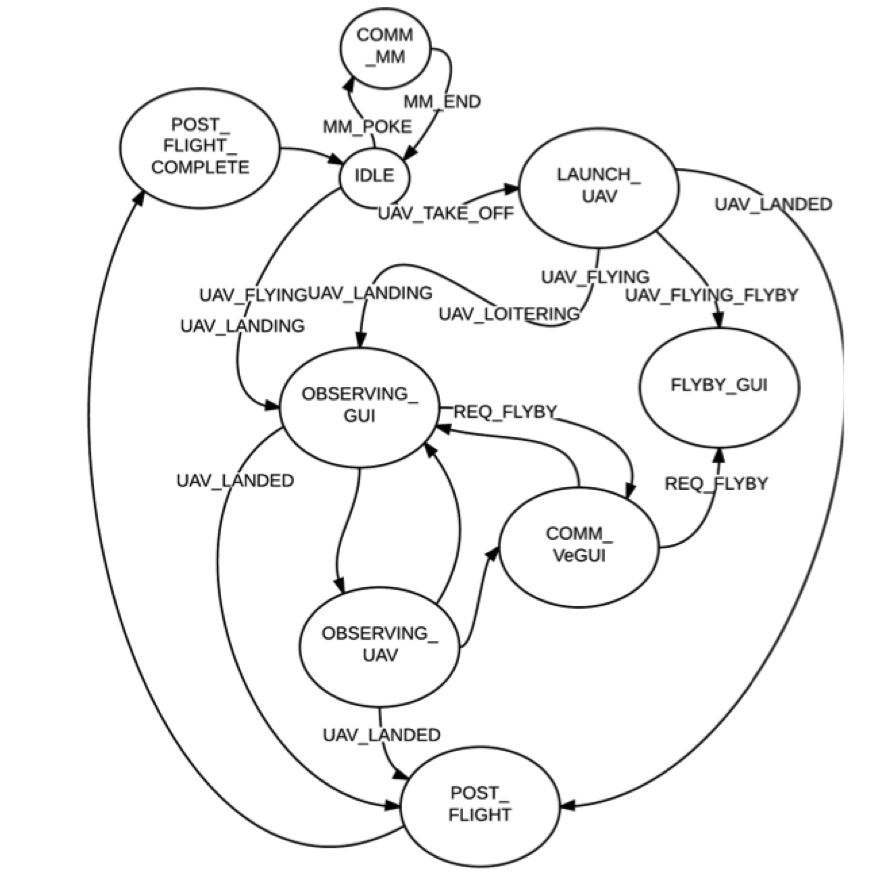
\includegraphics[height=2.4in]{DiRG.png}
\caption{Example actor model from prior work.}
\label{fig:dirg}
\end{figure}
\end{comment}

Actors represent the human decision-makers and autonomous elements of the WiSAR team.  An actor is composed of a set of states $S$, an initial state $s_0$, a set of inputs from the environment $\Sigma_{\rm env}$, a set of inputs from other actors on the team $\Sigma_{\rm team}$, a set of outputs $\Lambda_{\rm out}$, a simple form of memory $\Omega_{\rm men}$, and a transition function that determines the next state from the inputs and memory $\delta$. Formally, we denote an actor as:
\begin{equation}
 	Actor = (S, s_0, \Sigma_{\rm env}, \Sigma_{\rm team}, \Lambda_{\rm out}, \Omega_{\rm mem},\delta)
 \label{eq:actor}
 \end{equation}

 An actor's output has two components: signals to other actors on a team and a {\em duration} parameter that represents the time required for the actor to complete its transition to the next state.  Thus, $\Lambda_{\rm out}=\Sigma_{\rm team} \times \mathbb{N}^+$.
Relative task difficulty is expressed by the duration of the transition.
%The duration represents the relative difficulty of the task(s) associated with the transition.
We justify this by assuming that all tasks are performed at a constant rate, thus more difficult tasks take longer.
 A transition is a relation on the cross product of inputs with outputs where the brackets separate inputs from outputs.
\begin{equation}
 \delta:[S\times\Sigma_{\rm env}\times\Sigma_{\rm team}\times\Omega_{\rm mem}] \times [S\times \Sigma_{\rm team} \times \Omega_{\rm mem}], 
\end{equation} 
 
Given an actor's current state, set of input signals, and memory, it is possible for multiple transitions to be possible.  This occurs because we assume that multiple environment signals or inter-actor signals may be occurring at the same time, which are all perceived by the actor since we assume perception is a parallel operation.  Thus, it is useful to explicitly note the number of transitions that are possible from a given state.   A transition is considered {\em enabled} when all of its input
requirements are met and {\em disabled} otherwise. 

When an actor is in a given state, it is useful to explicitly denote the set of enabled and disabled transitions.  This information enables an estimate of algorithmic workload, where we assume that algorithmic workload is a function of the number of choices available to the actor.  Thus, we allow the current state to give a workload signal
\begin{equation}
	s_0^{\rm work\  sig} = (T_{enabled}, T_{disabled}) : T_{enabled} \cap T_{disabled} = \emptyset
 \label{eq:state}
\end{equation}

Internal variables within an actor are comprised of facts stored by an actor and used in decision making.
%Internal facts stored by an actor and used in decision making take the form of internal variables within an actor.
A good example of this can be seen in the mission manager actor of our simulation. As the search begins, the mission manager receives a number of data items from the parent search, e.g. search area and target description. These items of information need to be communicated separately to different actors, so they must be stored internally in the mean time. 

\section{Directed Team Graph (DiTG)}

A key element of the actors is that inputs to one actor can be outputs from another actor.  We can therefore create a directed graph from actor to actor, with an edge from actor~A to actor~B existing if the output from actor~A is a possible input to actor~B.  We call this graph a {\em Directed Team Graph} (DiTG); Figure~\ref{fig:ditg} illustrates the DiTG for the WiSAR team used in this paper.   

Using the fact that multiple resource theory indicates that visual and auditory channels can be perceived in parallel \cite{wickens2002multiple}, it is useful to label the edges in the graph with the {\em channel type} as in Figure~\ref{fig:ditg_detail}.  These labels allow the model-checker to identify when multiple signals are given to a single actor over the same channel.  When this occurs, we expect actor workload to be high.

%We hope to gain
%insight into decreasing the system workload, and possibly combining roles, by
%establishing metrics associated with the system model and model simulation. 
%These metrics can then be used to determine if changes to the model represent a
%decrease in operator workload.

\begin{figure}[h]
\center
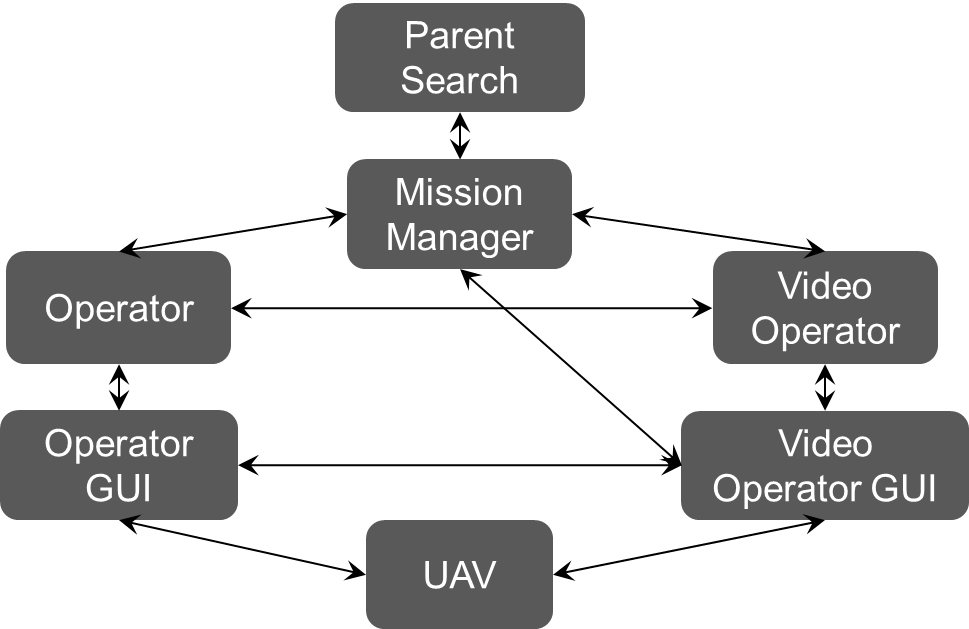
\includegraphics[width=4in]{ditg.png}
\caption{High Level DiTG}
\label{fig:ditg}
\end{figure}

\begin{figure}[h]
\center
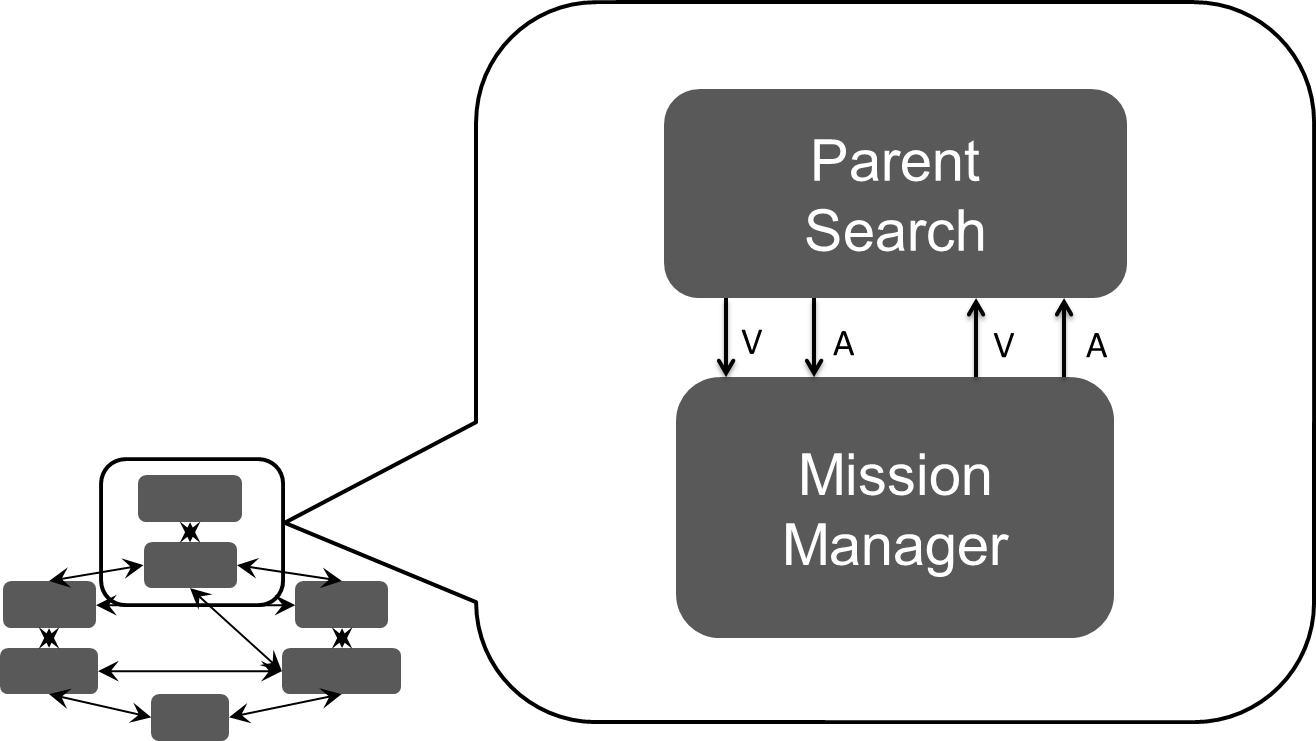
\includegraphics[width=4in]{ditg_detailed.png}
\caption{Detail view of DiTG: V is a Visual channel and A is an Audio channel}
\label{fig:ditg_detail}
\end{figure}

%Formally, the framework is the following mathematical structures:
% \begin{equation}
% 	DiTG = (A, \Phi, \forall a_i \in A~ \exists \Phi_i \subset \Phi)
% \end{equation}

% \begin{equation}
% 	Actor = (S, s_0, s_{current}, \Omega_A, \Sigma_A \subset \Phi, \Lambda_A
% 	\subset \Phi)
 %\label{eq:actor}
 %\end{equation}
%
% \begin{equation}
%	State = (T_{enabled}, T_{disabled}) : T_{enabled} \cap T_{disabled} = \emptyset
% \label{eq:state}
%\end{equation}
%
%\begin{equation}
%\begin{split}
%	Transition = (\Omega_{input} \subset \Omega_A, \Sigma_{input} \subset \Sigma_A,\\
%	\Omega_{value}^{input}, \Sigma_{value}^{input} \\
%	\Omega_{output} \subset \Omega_A, \Lambda_{output} \subset \Lambda_A, \\
%	\Omega_{value}^{output}, \Lambda_{value}^{output}, duration)
% \label{eq:transition}
% \end{split}
%\end{equation}

%\begin{equation}
%\begin{split}
%Channel (\phi) = (type \in (visual, audio), \\
%value \in (null, *), 
% a_i^{source}, a_j^{target}) : i \neq j
% \label{eq:channel}
% \end{split}
%\end{equation}
%
%\begin{equation}
%Declarative Memory(\omega) = value \in (null, *)
%\end{equation}


%\noindent where $A$ is a set of actors, $S$ a set of
%states, $T$ a set of transitions, $\Phi$ a set of channels, $\Omega$ a set of
%declarative memory, $\Sigma$ a set of input channels, and $\Lambda$ a set of
%output channels.

We represent a system as a DiTG, a collection of
actors connected to one another by a set of channels.  Whenever the state of the
system changes, an actor will petition from its current state, a list of enabled
transitions thus defining what decisions can be made.  The actor may then
activate one of these transitions.  

Since transitions from one state to another take time, as encoded in the {\em Duration} element of the output, it is useful to label transitions as either {\em active} or {\em fired}. Transitions in the actor model are labeled as {\em enabled} and {\em disabled}. When we consider the workload of an actor as part of the overall team, workload depends on what is going on with other team members, so we add the active and fired labels in order to determine when an enabled transition (meaning a possible choice available to an actor) is chosen by an actor (making it active) and when the actor completes the work required to enter the next state (the transition fires).  

From an implementation perspective, when a transition becomes active it creates temporary
output values for declarative memory and channels.  These temporary values are
then applied to the actual declarative memory and channel values once the transition fires.

For our model we never explicitly define a single task.  Instead
we define actors, states, and transitions.  Each transition defines its own
perceptual, cognitive, response, and declarative resources \cite{salvucci2008threaded}, allowing the model to represent multiple possible tasks.\footnote{Grant, Kraus, and Perlis have done exceptional work compiling formal approaches
to teamwork. While the formalisms are not explicit in our modeling, our informed
modelers apply these approaches. For example, joint intentions are represented
in actors containing complement transitions.}  In this way, an actor's state
determines what task(s) are being performed, achieving multi-tasking without
explicitly defining tasks. 

%\subsection{Model Creation}
%To simplify the modeling process and ensure rigorous model creation we
%developed a transition language, similar to a Kripke structure, which allows
%models to be expressed as a list of Actor transitions.  A parser then
%automatically generates the classes required to run the model simulation.
%The transition language uses the following structure.
%\begin{equation}
%\begin{split}
%(s_{current}, [\phi_{input} = value,\ldots], [\omega_{input} = value,\ldots],\\
%duration) \times \\
%(s_{next}, [\phi_{output} =
%value,\ldots], [\omega_{output} = value,\ldots])
%\end{split}
%\end{equation}
%\noindent The language is compiled to a Java program suitable to run standalone
%as a simulation or analyzed by the JPF model checker to create
%workload profiles.


To simplify the modeling process and ensure rigorous model creation we
developed a transition language, similar to a Kripke structure,\footnote{Since our purpose behind building a model was to allow us to examine workload we decided against using standard model checkers such as Spin since they did not provide the same level of flexibility that we obtained via java and JPF.}  which allows
models to be expressed as a list of Actor transitions.  A parser then
automatically generates the classes required to run the model simulation.
The transition language uses the following structure.
\begin{equation}
\begin{split}
(s_{current}, [\phi_{input} = value,\ldots], [\omega_{input} = value,\ldots],\\
duration) \times \\
(s_{next}, [\phi_{output} =
value,\ldots], [\omega_{output} = value,\ldots])
\end{split}
\end{equation}
\noindent The language is compiled to a Java program suitable to run standalone
as a simulation or analyzed by the JPF model checker to create
workload profiles.

\section{Workload Metrics}

We are now in a position to combine the three categories of workload (cognitive, algorithmic, and temporal) with the formal model of the actors and team to generate a set of workload metrics.  Because the categories include many possible measurements that are beyond the scope of this paper, we use labels for the workload metrics that are slightly different from the workload categories.  As shown in Figure~\ref{fig:WorkloadMetrics}, cognitive workload or resource workload as it is termed in this work, is measured using metrics under the {\em resource} workload label, algorithmic under {\em decision}, and temporal workload is labeled the same. 


\begin{figure}[h]
\center
\setlength{\abovecaptionskip}{1mm}
\setlength{\belowcaptionskip}{1mm}
\setlength{\textfloatsep}{1mm}
\setlength{\floatsep}{1mm}
\scalebox{.8}{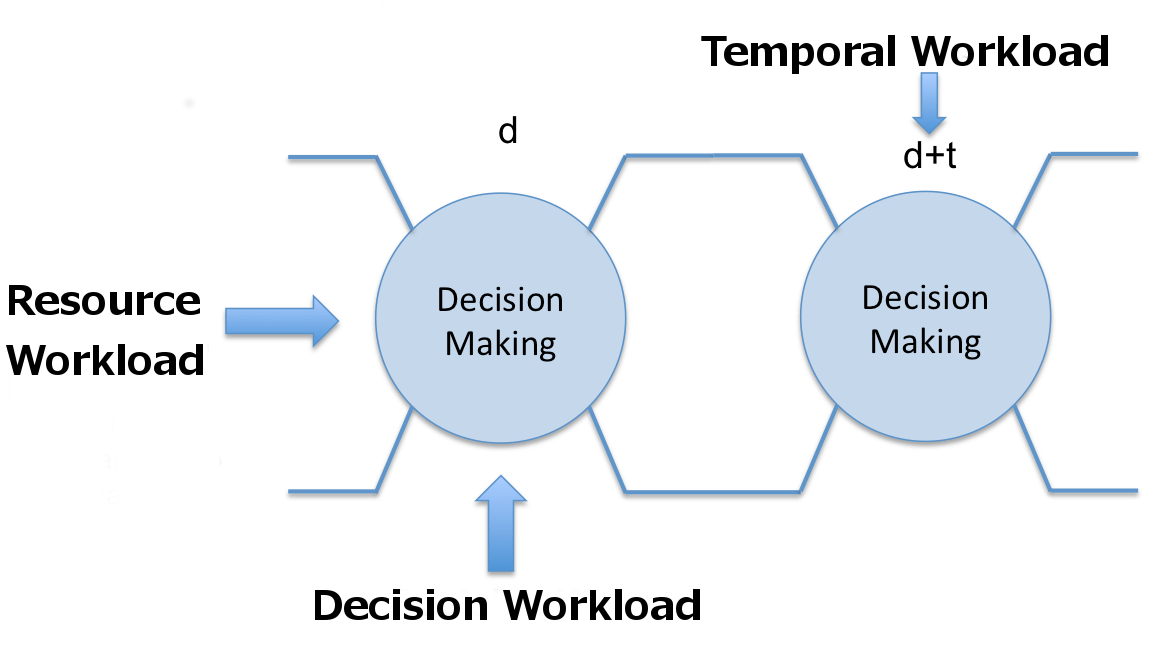
\includegraphics[height=2.5in]{WorkloadMetrics.png}}
\caption{Workload in the model.}
\label{fig:WorkloadMetrics}
\end{figure}

Resource workload is separated into both inter-actor communication and actor
memory load. Decision workload can be broken down into timing, algorithm complexity, and complexity of the solution. Temporal workload includes operations tempo, arrival rate, and response time.

Java Pathfinder (JPF) is a tool used to explore all points of nondeterminism.
%find all possible paths represented in Java source code. 
It does this by compiling the source code as a JPF binary and
running it in a virtual machine.
Sections of the program are then dynamically altered 

The virtual machine can dynamically alter sections of the program and concurrently generate and run copies of the program
based off of these changes. This allows us to include alterable values in our
model and simulate an array of different actors without the need to modify the
model.

We have set up a JPF listener to record workload. A JPF listener is a tool that
follows the Listener Design Pattern and acts in the expected fashion. We have
focused our listeners on three pieces of the model: the active inputs, enabled
transitions, and the time taken to perform a transition. We then use these
pieces of the model to represent resource, decision, and temporal workload respectively.

\section{Results}

In the interest of consolidating operators it is critical to find an accurate measurement that detects situations that exceed the capacity of a given human. One way to detect this is by building a map of each actor's workload as a function of time. JPF explores all possible paths the model can take and returns the ones that violate the model's criteria. By augmenting our model with the workload metrics we can identify all possible areas of high workload. 

We propose three levels of increasing validity for evaluating the approach in the paper.  The first level, the one used in this paper, is to check for {\em consistency}.  We say that the approach is {\em consistent} if the workload peaks, valleys, and trends match what we know about a small set of given situations; in other words, the approach is consistent if it matches our expectations on tasks that we know a lot about.  

The second level, which is an area for future work, is to check for {\em sensitivity}.  We say that  the approach is sufficiently {\em sensitive} if we can use JPF to find new scenarios that have very high or very low workloads, and we can then generate a satisfactory explanation for the levels of workload by evaluating the new scenarios.  The third level, another area of future work, is to {\em substantiate} workload levels using experiments with human participants by comparing the perceived workload of humans with those predicted by the model.

In this paper, we restrict attention to finding areas of high and low workload, and then checking these areas for consistency.  We evaluated consistency using two scenarios.  The first is when the Video Operator was able to identify the target during a flight without any complications occurring (see Figure~\ref{fig:WorkloadSim1}). As the workload measure currently does not have units, the plots are normalized in each category. For the first 40 time steps everything behaves as expected with low to moderate workload. An initial workload bump occurs as actors exchange information necessary to start a search.   At time step forty we see a dramatic deviation from the norm. This deviation is a result of constant information passing between the GUIs and the operators
making it only
%. Since there is a constant passing of data between the machinery and the operators, it is only
 logical that the workload would increase substantially.

\begin{figure}[h]
\center
\setlength{\abovecaptionskip}{1mm}
\setlength{\belowcaptionskip}{1mm}
\setlength{\textfloatsep}{1mm}
\setlength{\floatsep}{1mm}
\scalebox{.9}{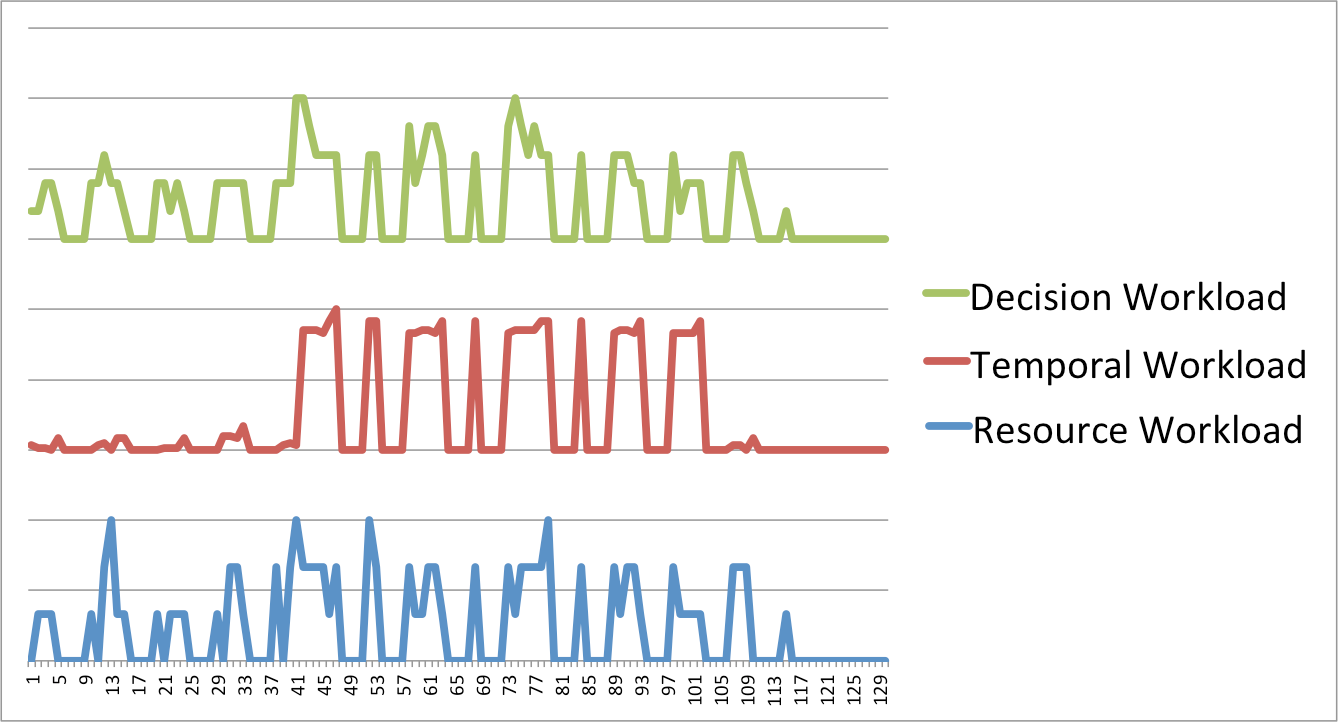
\includegraphics[height=2in]{WorkloadTargetSightingLabeled.png}}
\caption{Workload over an uneventful flight.}
\label{fig:WorkloadSim1}
\end{figure}

The second simulation is a scenario where after a short period of flight the battery rapidly fails. In this particular situation, the operator was unable to respond quickly enough to land the UAV before it crashed (see Figure~\ref{fig:WorkloadSim2}). There is an immediate spike in the temporal workload (middle plot), but surprisingly, the workload then decreases back to normal levels in just five time steps.
The second spike revealed an unexpected fluctuation workload leading us to reexamine how information was reported. We found that there was an error in the simulator that has since been repaired.
%The second spike indicates an unexpected fluctuation in options among one of the actors, which will have to be investigated further to verify if this is an accurate response or if a flaw in the model had slipped past the verification stage of development.
Finally, as would be expected, when the UAV crashed there was a small spike in the workload before everything came to a halt. 

\begin{figure}[h]
\center
\setlength{\abovecaptionskip}{1mm}
\setlength{\belowcaptionskip}{1mm}
\setlength{\textfloatsep}{1mm}
\setlength{\floatsep}{1mm}
\scalebox{.75}{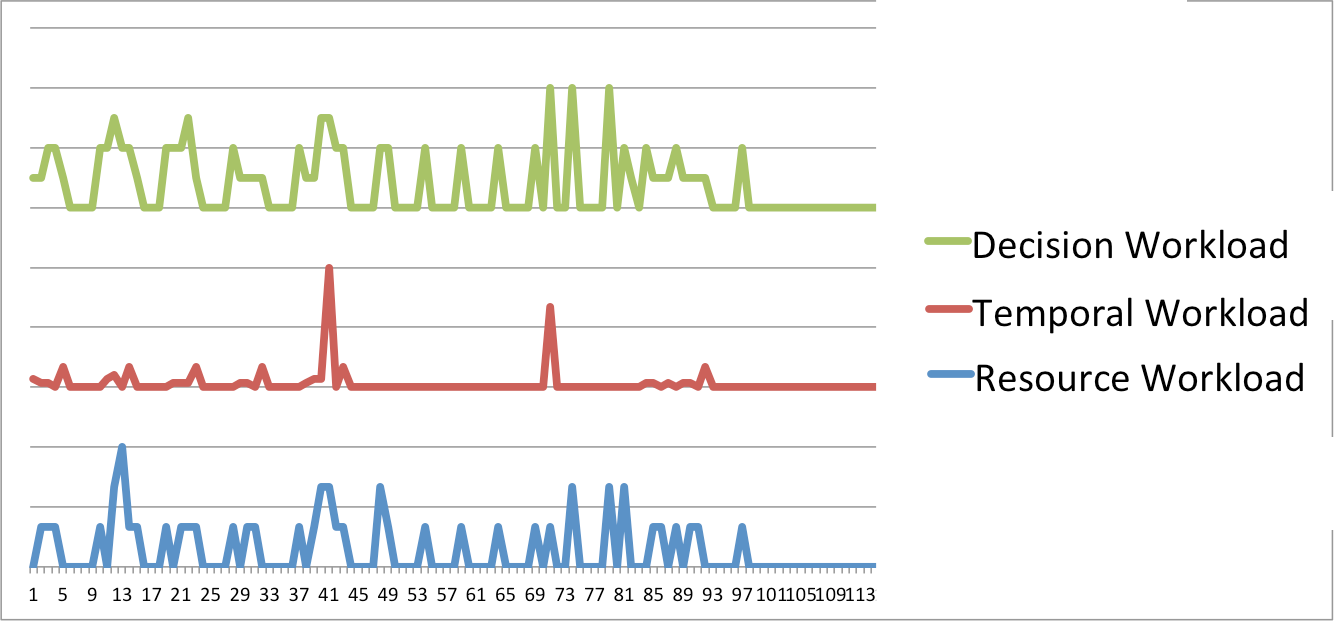
\includegraphics[height=2in]{WorkloadCrashedLabeled.png}}
\caption{Emergency battery failure simulation}
\label{fig:WorkloadSim2}
\end{figure}

\section{Related Work}

This work is an extension of previous work which focused on modeling human
machine systems, specifically WiSAR.  This work extends this model to
incorporate the measurement of workload~\cite{gledhill2013modelinguas}.

Multiple resource theory plays a key role in how we are measuring workload~\cite{wickens2002multiple}. The multiple resource model defines four categorical dimensions that
account for variations in human task performance.  A task can be represented as a vector of these dimensions.  Tasks interfere when they share resource dimensions.  Using these vectors, Wickens defined a basic workload measure consisting of the task difficulty (0,1,2) and the number of shared dimensions.  Using this metric it is possible to predict task interference by looking at tasks which use the same resource dimensions.  Our model differs in that we do not explicitly define tasks, instead we use Actor state transitions which may imply any number of concurrent tasks.  The transition then informs us of which resources are being used and for how long.  

Threaded cognition theory states that humans can perform
multiple concurrent tasks that do not require executive processes~\cite{salvucci2008threaded}.  By making a
broad list of resource assumptions about humans, threaded cognition is able to
detect the resource conflicts of multiple concurrent tasks.  Our model differs from
threaded cognition theory in that it does not allow learning nor does our model distinguish
between perceptual and motor resources. In almost all other aspects our model behaves in a similar fashion.

Related work on temporal workload has attempted to predict the number of UAVs an operator can
control, otherwise known as {\em fan-out}~\cite{cummings2007predicting,OlsenWood2004,CrandallEtAl2005}.  This work used queuing theory
to model how a human responds in a time sensitive multi-task environment.  Queuing theory is helpful in determining the temporal effects of task performance by measuring the difference between when a task was received and when it was executed.  Actors can only perform a single transition at a time, similar to queuing theory, but it is possible for each state to take input from multiple concurrent tasks which differs from standard models of queuing theory.

ACT-R is a cognitive architecture which attempts to model human cognition and
has been successful in human-computer interaction applications~\cite{anderson2004integrated,lebiere2013cognitive}.  The
framework for this architecture consists of modules, buffers, and a pattern-matcher which in many ways are very similar to our own framework.  The major
difference is that ACT-R includes higher levels of modeling detail, such as memory access
time, task learning, and motor vs perceptual resource differences.  Our model exists at a higher level of abstraction.

Complementary work has been done using Brahms.
%Brahms is a powerful language that allows for more detail than our research required.
Brahms is a powerful language that allows for far more detail than we found our research required.
In addition at the time we started developing our model Brahms lacked some of the tools we needed for extracting workload data from the model. Because of this we found that Java in conjunction with JPF made a better match for our needs.

\section{Summary and Future Work}

This paper proposes a model-checking approach to analyzing human workload in an UAS.  Humans and other autonomous actors are modeled as modified Moore machines, yielding a directed graph representing team communication.  Workload categories are distilled from the literature, and the models of the actors and team are augmented so that specific workload metrics can be obtained using model-checking.  Preliminary analysis demonstrates a weak level of validity, namely, that the temporal workload profile is consistent with expected behavior for a set of well-understood situations.  For these scenarios, inter-actor communication is a primary cause of spikes in workload. 

A sensitivity study, followed by an experiment with real human users is needed to understand and justify the workload measures. Once we have verified that our system analyzes workload correctly, it will be useful to design a GUI optimized to managing workload and to formulate a generalized model that will have application to other human-machine systems.


% use section* for acknowledgement
% use section* for acknowledgement
\section*{Acknowledgment}
% optional entry into table of contents (if used)
% \addcontentsline{toc}{section}{Acknowledgment}
The authors would like to thank the NSF IUCRC Center for Unmanned Aerial Systems, and the participating industries and labs, for funding the work.